% -------------------------------------------------------------------------------- %

\begin{exercise}[Implementation Task: 10 armed-testbed]

Implement a simple bandit algorithm for the ``10-armed-testbed''.
(Ten independent bandits whose action values $a_i$ is taken from a normal distribution
with mean $a_i$ and variance $1$.)

Repeat the experiment 1000 times steps and average over 1000 independent runs for at least
3 different epsilon values and plot the results.
\end{exercise}

% -------------------------------------------------------------------------------- %

\begin{solution}

\begin{figure}[H]
  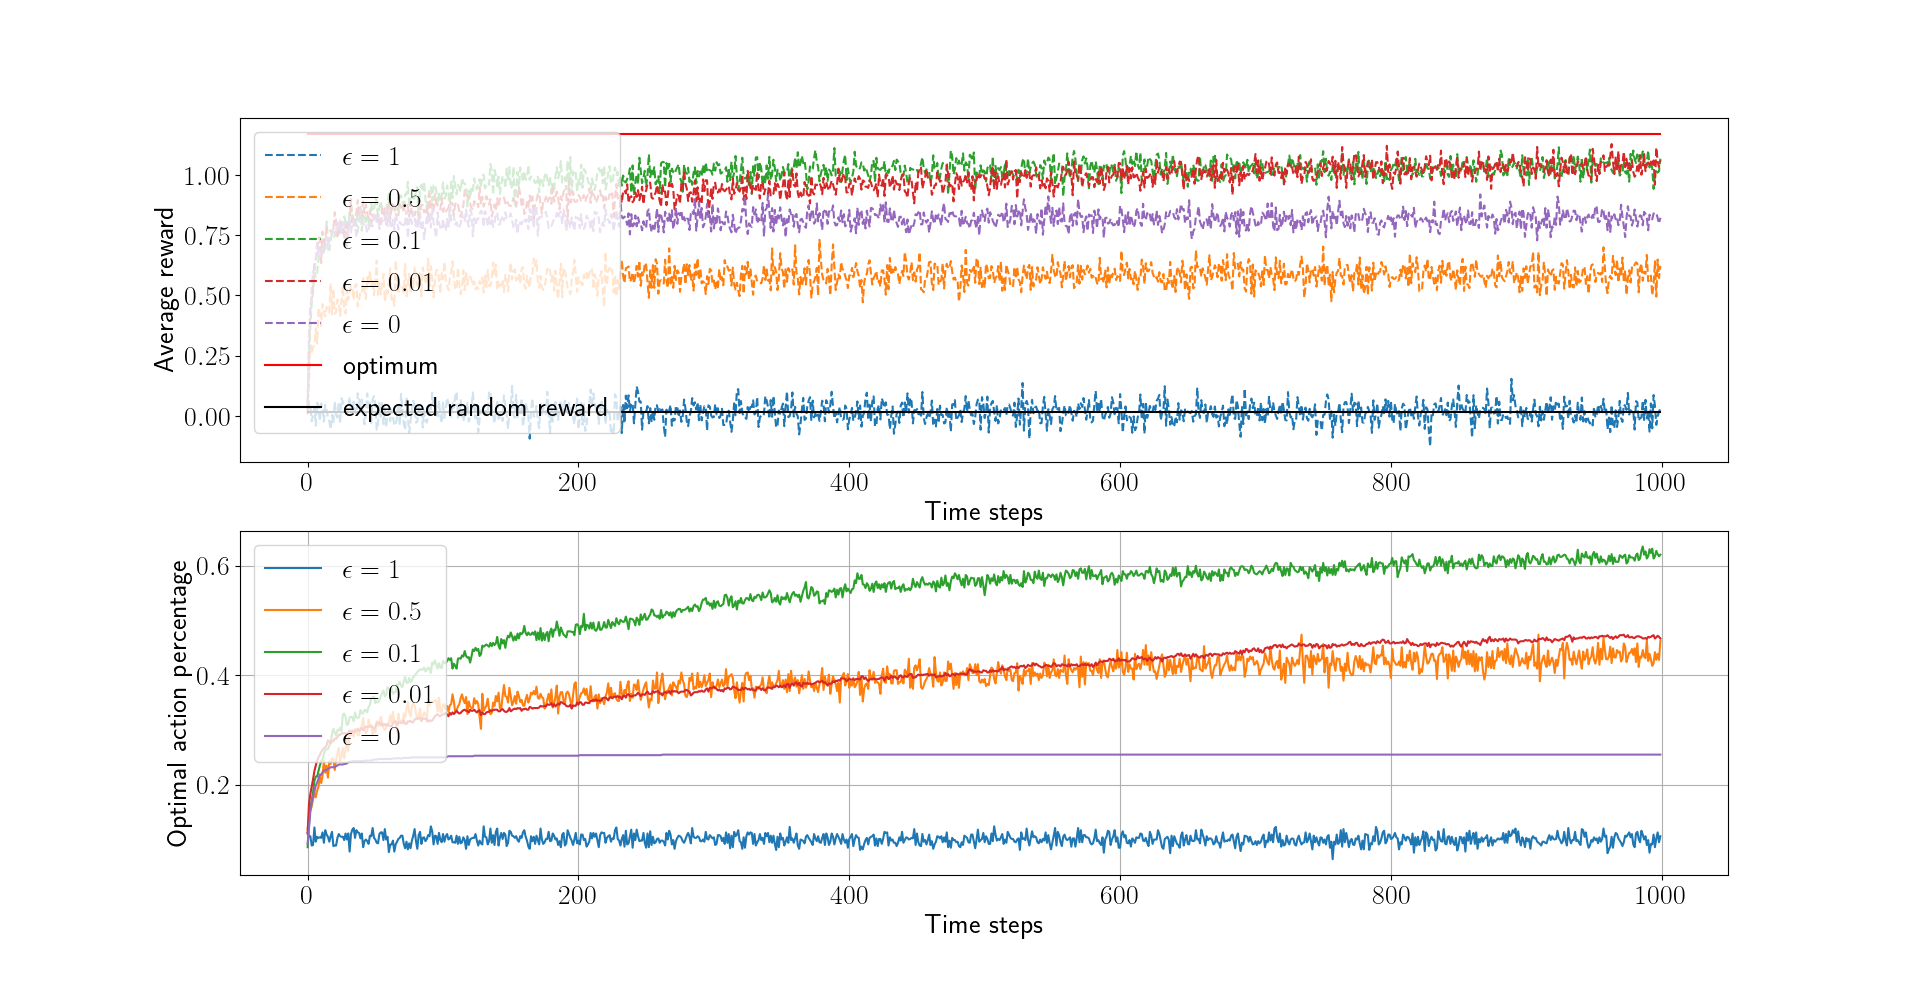
\includegraphics[width = \linewidth]{plot_1.4.png}
  \caption{Ergebnisse des Testlaufs}
  \label{fig:plot1}
\end{figure}

\end{solution}

% -------------------------------------------------------------------------------- %
